
% Chapter content only — insert with \input{customer_segmentation_chapter.tex}
\chapter{RFM Analysis and K-Means Clustering}\label{chap:ml}

\section{Motivation}

The CompanyX transactional database contains purchases from May 2011 through June 2014. However, raw sales records alone do not identify which customer groups require different business strategies. This chapter follows the team's implemented approach: summarize purchase behaviour using RFM, clean and transform the features, fit K-Means to customer snapshots, and translate the resulting numeric clusters into interpretable segment names. The trained configurations can then be reused by the operational scoring pipeline and historical snapshot process.

\subsection{RFM Variables}
Recency (R) is the number of days from an evaluation date to the customer's last purchase. Frequency (F) is the count of distinct sales orders within the trailing 365 days. Monetary (M) is the sum of order-line amounts within that same 365-day period. Recency may exceed 365 days for customers who have not purchased recently. The year-end training snapshots used by the project are 31 December 2011, 2012, and 2013; there is no 2014 trained model.

\section{Data Cleaning}

The raw data is first ingested from the FactCustomerSnapshot, and then processed through deduplication. After that, any
R, F, or M values are missing, the process stops and reports the number of affected rows to the ETL Team. Anomalies
values such as negative values are set to zero, since a purchase count or a monetary value can not be negative.

This subset of data serves a representative overview of customer purchases based on RFM analysis as mentioned above.

\begin{table}[htbp]
  \centering
  \small
  \begin{tabular}{rrrr}
    \hline
    \textbf{Customer} & \textbf{Recency} & \textbf{Frequency} & \textbf{Monetary} \\
    \hline
    11057             & 37               & 1                  & 3729.36           \\
    11058             & 22               & 1                  & 3756.99           \\
    11060             & 12               & 1                  & 3756.99           \\
    11061             & 18               & 1                  & 3729.36           \\
    11072             & 0                & 1                  & 3756.99           \\
    11238             & 84               & 1                  & 3756.99           \\
    11239             & 71               & 1                  & 3729.36           \\
    11240             & 32               & 1                  & 3756.99           \\
    11243             & 38               & 1                  & 3756.99           \\
    11244             & 47               & 1                  & 3756.99           \\
    11247             & 41               & 1                  & 3729.36           \\
    11250             & 14               & 1                  & 3756.99           \\
    11333             & 10               & 1                  & 3756.99           \\
    11334             & 27               & 1                  & 3756.99           \\
    11337             & 22               & 1                  & 3729.36           \\
    11591             & 79               & 1                  & 3953.99           \\
    11592             & 79               & 1                  & 3953.99           \\
    11593             & 69               & 1                  & 3953.99           \\
    11599             & 72               & 1                  & 3953.99           \\
    11601             & 71               & 1                  & 3953.99           \\
    11606             & 82               & 1                  & 3953.99           \\
    11607             & 71               & 1                  & 3953.99           \\
    \hline
  \end{tabular}
  \caption{Example RFM records before preprocessing.}\label{tab:rfm_sample}
\end{table}

\section{Log transformation}

Spending and purchase counts are usually right-skewed. Most customers spend a moderate amount, while only a small
number spend many times more. If raw values are used, these large values stretch the scale and the K-Means model spends
more effort unnecessarily separating a few high spenders (outliers) rather than grouping typical customers. By using
log transformation, the issue can be minimized.

For example, a customer who spends 3,000 and 300,000 differs by a factor of 100 in raw terms, but their log values
differ by only 4.6. We use log(1+x) in this case, written log1p because some customers have a value of zero, which
leads to log(0) undefined.

\begin{table}[htbp]
  \centering
  \small
  \begin{tabular}{rrrr}
    \hline
    \textbf{Customer} & \textbf{Recency} & \textbf{Frequency} & \textbf{Monetary} \\
    \hline
    11057             & 3.638            & 0.693              & 8.224             \\
    11058             & 3.135            & 0.693              & 8.232             \\
    11060             & 2.565            & 0.693              & 8.232             \\
    11061             & 2.944            & 0.693              & 8.224             \\
    11072             & 0.000            & 0.693              & 8.232             \\
    11238             & 4.443            & 0.693              & 8.232             \\
    11239             & 4.277            & 0.693              & 8.224             \\
    11240             & 3.497            & 0.693              & 8.232             \\
    11243             & 3.664            & 0.693              & 8.232             \\
    11244             & 3.871            & 0.693              & 8.232             \\
    11247             & 3.738            & 0.693              & 8.224             \\
    11250             & 2.708            & 0.693              & 8.232             \\
    11333             & 2.398            & 0.693              & 8.232             \\
    11334             & 3.332            & 0.693              & 8.232             \\
    11337             & 3.135            & 0.693              & 8.224             \\
    11591             & 4.382            & 0.693              & 8.283             \\
    11592             & 4.382            & 0.693              & 8.283             \\
    11593             & 4.248            & 0.693              & 8.283             \\
    11599             & 4.290            & 0.693              & 8.283             \\
    11601             & 4.277            & 0.693              & 8.283             \\
    11606             & 4.419            & 0.693              & 8.283             \\
    11607             & 4.277            & 0.693              & 8.283             \\
    \hline
  \end{tabular}
  \caption{Log-transformed sample RFM values.}
\end{table}

\section{Standardization}

Before importing data to run the K-Means Clustering model, it is essential to standardize the RFM values to ensure that
each metric contributes equally to the analysis, since Recency, Frequency, and Monetary values are measured on
different scales. K-Means relies heavily on distances (later will be shown), so a variable with a larger spread would
dominate the result.

StandardScaler solves this by subtracting the mean and dividing by the standard deviation of each variable, so that
each one has a mean of 0 and a standard deviation of 1. The mean and standard deviation are estimated from the training
data and stored, so that new customers are scaled in the same way.

\begin{table}[htbp]
  \centering
  \small
  \begin{tabular}{rrrr}
    \hline
    \textbf{Customer} & \textbf{Recency} & \textbf{Frequency} & \textbf{Monetary} \\
    \hline
    11057             & 0.109            & 0.000              & -0.875            \\
    11058             & -0.392           & 0.000              & -0.581            \\
    11060             & -0.962           & 0.000              & -0.581            \\
    11061             & -0.583           & 0.000              & -0.875            \\
    11072             & -3.522           & 0.000              & -0.581            \\
    11238             & 0.913            & 0.000              & -0.581            \\
    11239             & 0.747            & 0.000              & -0.875            \\
    11240             & -0.032           & 0.000              & -0.581            \\
    11243             & 0.135            & 0.000              & -0.581            \\
    11244             & 0.342            & 0.000              & -0.581            \\
    11247             & 0.209            & 0.000              & -0.875            \\
    11250             & -0.819           & 0.000              & -0.581            \\
    11333             & -1.128           & 0.000              & -0.581            \\
    11334             & -0.196           & 0.000              & -0.581            \\
    11337             & -0.392           & 0.000              & -0.875            \\
    11591             & 0.852            & 0.000              & 1.454             \\
    11592             & 0.852            & 0.000              & 1.454             \\
    11593             & 0.719            & 0.000              & 1.454             \\
    11599             & 0.761            & 0.000              & 1.454             \\
    11601             & 0.747            & 0.000              & 1.454             \\
    11606             & 0.889            & 0.000              & 1.454             \\
    11607             & 0.747            & 0.000              & 1.454             \\
    \hline
  \end{tabular}
  \caption{Standardized sample RFM values.}
\end{table}

\section{K-Means Clustering}

K-Means is an unsupervised algorithm that partitions observations into \(K\) clusters by iteratively assigning each point to the nearest centroid and updating centroid locations. The project fits scikit-learn \texttt{KMeans} with \(K=5\), \texttt{k-means++} initialization, \texttt{n\_init=10}, \texttt{max\_iter=300}, and \texttt{random\_state=42}.

For each data point in the dataset, calculate the Euclidean distance between the point and each centroid. Assign the
data point to the cluster with the closest centroid

\[ d(\mathbf{x},\mathbf{c}) = \sqrt{\sum_{j=1}^{3} (x_j-c_j)^2}. \]

Where:
\begin{itemize}
  \item $d(x, y)$: the distance between data point x and centroid y
  \item $y_i$: donates the value of the i-th attribute value of centroid y
  \item $x_i$: represents the i-th attribute of the data point x
  \item $i$ : refers to index of the attribute
  \item $n$ : indicates the total number of the attribute for each data point
\end{itemize}

Within-cluster sum of squares (WCSS), also called inertia, measures the total squared distance from observations to their assigned centroids:

\[ \mathrm{WCSS}=\sum_{k=1}^{K}\sum_{i\in S_k}\sum_{j=1}^{3}(x_{ij}-c_{kj})^2. \]

Where:
\begin{itemize}
  \item K: Total number of clusters.
  \item k: An index that refers to the current cluster, ranging from 1 to K.
  \item $S_k$: The set of data points assigned to cluster k.
  \item p: Number of features or dimensions in the dataset.
  \item j: An index that refers to the current feature or dimension, ranging from 1 to p.
  \item $x_{ij}$: The j-th feature value of the i-th data point.
  \item $\bar{x}_{kj}$: The mean value of the j-th feature in cluster k (i.e., the centroid's value).
  \item $(x_{ij} - \bar{x}_{kj})^2$: The squared Euclidean distance between the j-th feature of data point xi and the corresponding feature of the centroid of its cluster.
\end{itemize}

This WCSS can also be known as the Inertia, the lower means the tighter the data points are grouped. Another important
criteria, which is Silhouette, also needs to be considered. The silhouette score measures how well-separated and
cohesive clusters are in K-Means clustering. It evaluates each data point's fit relative to its own cluster versus
neighboring clusters.

Figures~\ref{fig:elbow_2013} and~\ref{fig:silhouette_2013} reproduce the diagnostic plots already saved with the project for the 31 December 2013 snapshot. Inertia decreases as \(K\) increases, while the silhouette metric measures separation between clusters. The silhouette score for \(K=5\) is approximately 0.518; \(K=2\) achieves a higher score (approximately 0.636) on this snapshot. Therefore five clusters were chosen as a \emph{business-interpretability trade-off}, supported by the elbow/silhouette diagnostics and the desire for distinct actionable customer profiles, not because five globally maximizes the silhouette score.

\begin{figure}[htbp]
  \centering
  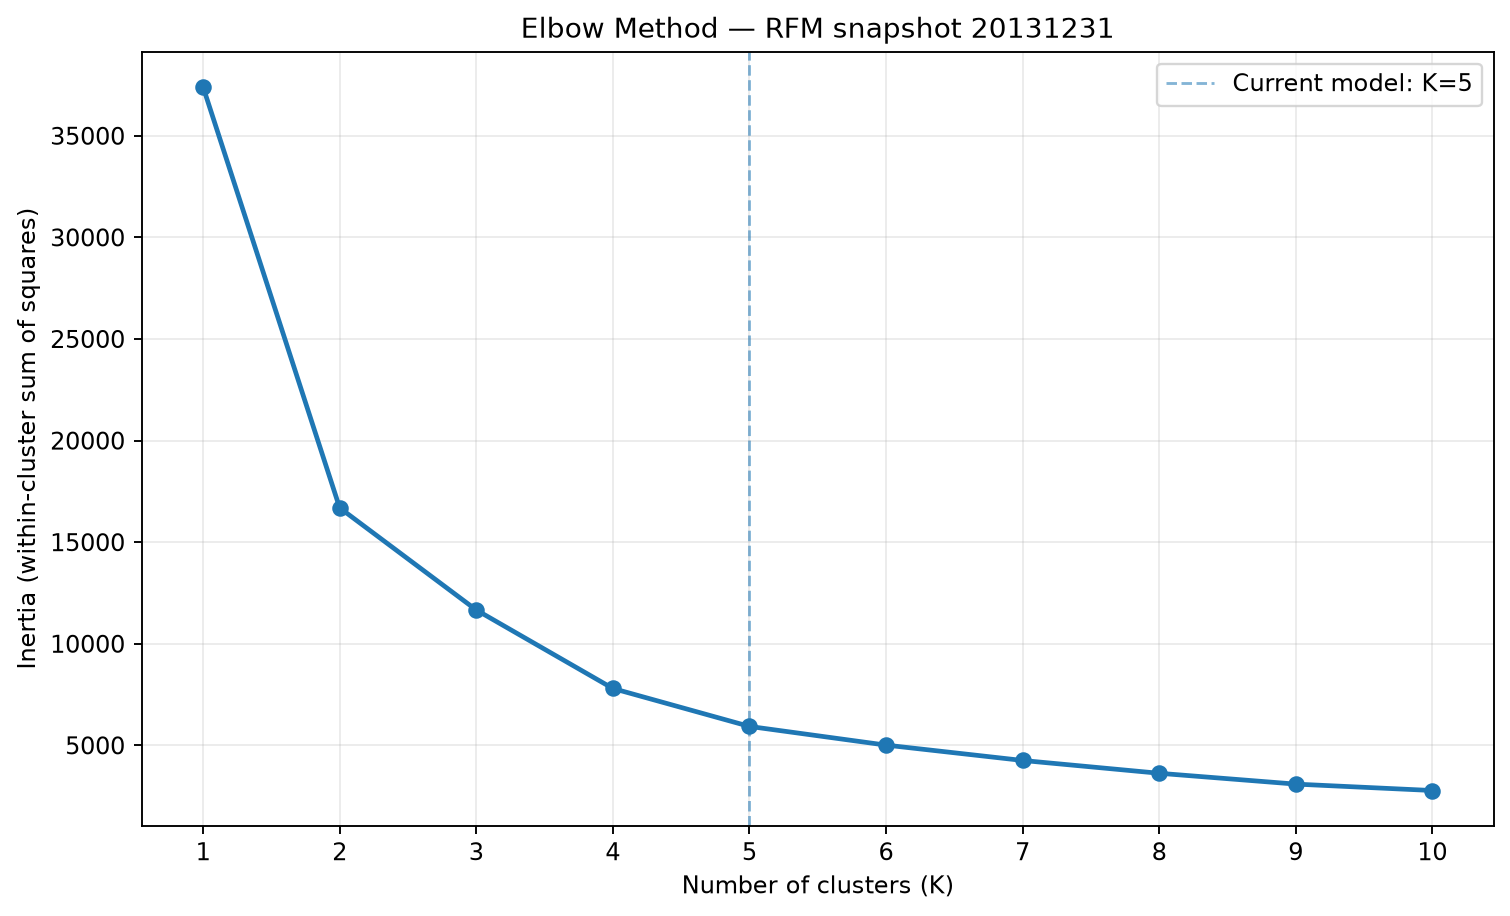
\includegraphics[width=0.94\textwidth]{elbow_20131231.png}
  \caption{Elbow plot for the 31 December 2013 RFM snapshot (existing project diagnostic).}
  \label{fig:elbow_2013}
\end{figure}
\begin{figure}[htbp]
  \centering
  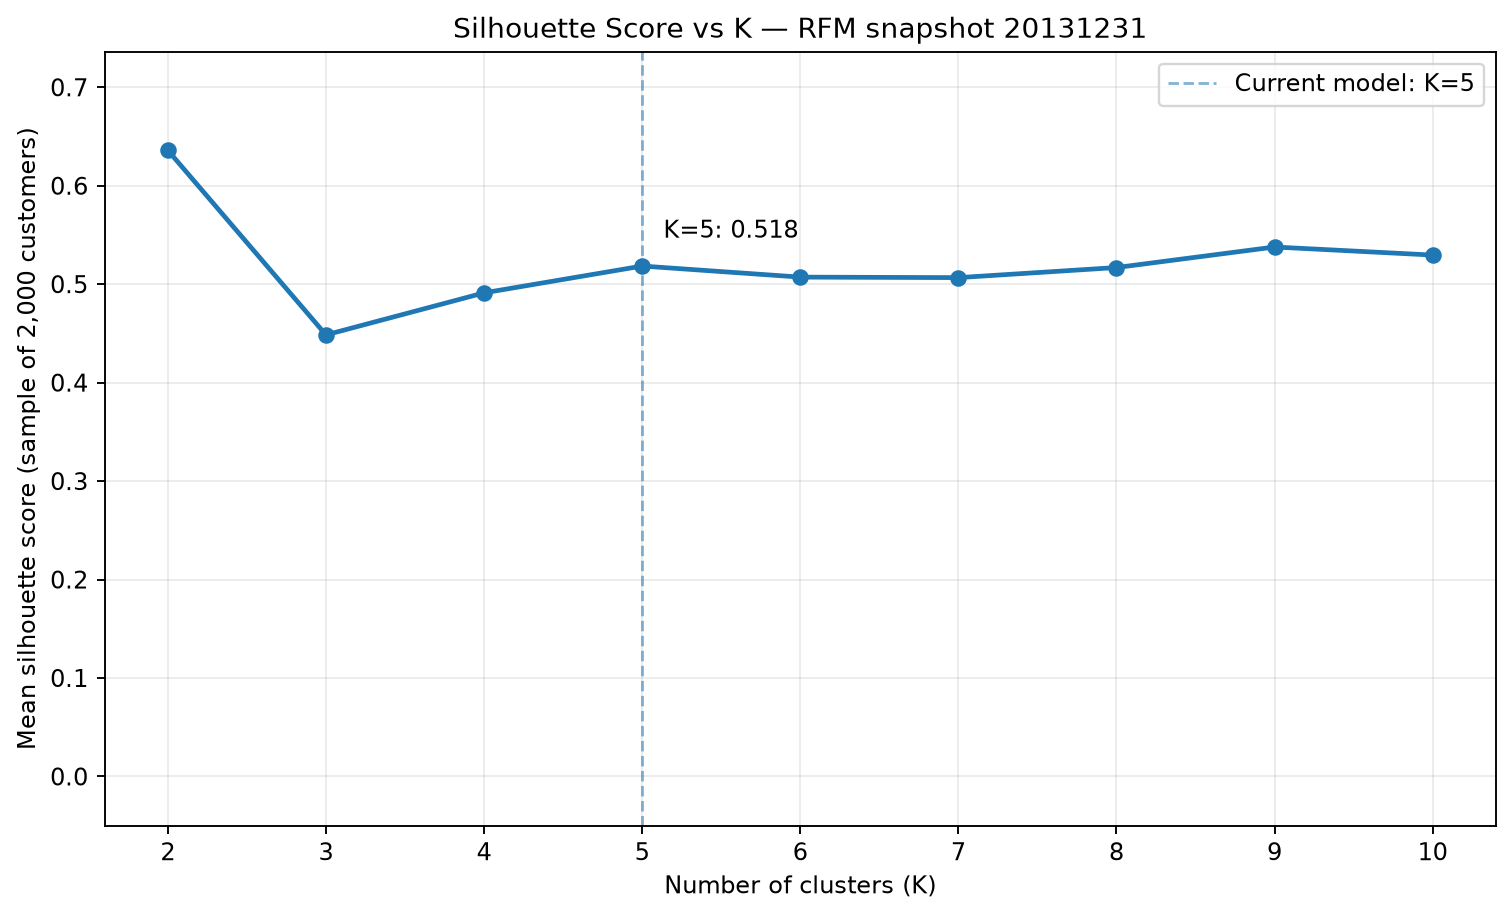
\includegraphics[width=0.94\textwidth]{silhouette_vs_k_20131231.png}
  \caption{Silhouette comparison for different cluster counts on the same snapshot.}
  \label{fig:silhouette_2013}
\end{figure}

K-Means only returns a numeric cluster ID (0 to 4) for each customer, which reflects no value of what the groups mean. Moreover,
annually the model is retrained and the number from 0 to 4 is different and not staying consistent. Therefore, to turn
them into meaningful clusters automatically, a solution is implemented: Each cluster on an RFM variable is given
``points'', based on how its average compares with the other clusters. The rules are

For Monetary and Frequency: the cluster with the highest average gets 5 points and the lowest get 1. (the higher these
values are, the more valuable they are)

For Recency: the rule is reversed because shorter time since the last purchase is better.

\noindent The implemented composite score is \(\text{Monetary rank}+\text{Frequency rank}+1.1\times\text{Recency rank}\).

Recency is weighted slightly higher, because a recent purchase is a strong sign that a customer is still active. Points
are given to clusters, not to individual customers.

The outcome will look like this:

\begin{table}[htbp]
  \centering
  \begingroup
  \scriptsize
  \setlength{\tabcolsep}{2pt}
  \begin{tabular}{rrrrrrrrl}
    \hline
    \textbf{Cluster} & \shortstack{\textbf{Avg}\\\textbf{Recency}} & \shortstack{\textbf{Avg}\\\textbf{Frequency}} & \shortstack{\textbf{Avg}\\\textbf{Monetary}} & \textbf{R points} & \textbf{F points} & \textbf{M points} & \textbf{Score} & \textbf{Segment}         \\
    \hline
    4                & 110.34                                      & 2.55                                          & 1,694.00                                     & 4                 & 5                 & 5                 & 14.4           & Champions                \\
    2                & 13.31                                       & 1.24                                          & 96.10                                        & 5                 & 4                 & 3                 & 12.5           & Recent / Promising       \\
    0                & 174.17                                      & 1.00                                          & 1,518.38                                     & 3                 & 2                 & 4                 & 9.3            & High-Value / Cooling Off \\
    3                & 196.03                                      & 1.03                                          & 48.91                                        & 2                 & 3                 & 2                 & 7.2            & Low-Spend / Occasional   \\
    1                & 602.92                                      & 0.00                                          & 0.00                                         & 1                 & 1                 & 1                 & 3.1            & Lost / Dormant           \\
    \hline
  \end{tabular}
  \endgroup
\end{table}

The example model output was recorded for an 18,484-customer analysis extract. The final dashboard chapter reports 18,485 customers for its June 2014 view. This one-record difference has not been reconciled in the submitted materials, so the two counts should not be presented as an identical population without verification.

Champions (cluster 4) has the highest frequency and spend, with an average of 2.55 purchases and 1,694 in total. Its
average recency is 110 days, so these customers are valuable but have not bought recently.

High-Value / Cooling Off (cluster 0) is the second-largest group by spend, but each customer has bought only once on
average. Their last purchase was about 174 days ago, so they are at risk of leaving.

Low-Spend / Occasional (cluster 3) is the largest group. Customers buy about once, spend about 49 on average, and last
bought about 196 days ago.

Recent / Promising (cluster 2) bought most recently, with an average of 13 days since the last purchase. Their spend is
low so far, which suggests they are new customers who may grow.

Lost / Dormant (cluster 1) has no recorded frequency or spend in the period, and an average recency of 603 days. These
customers have stopped buying.

\section{Conclusion}

The result of the RFM Analysis and K-Means clustering reveal the distinct customer segments with unique purchasing
behaviours. By standardizing the RFM variables and applying the K-Means algorithm, the dataset was successfully divided
into five interpretable clusters. Such segmentation highlights not only the diversity in customer engagement levels but
also provides valuable insights for strategic business decision-making. Therefore, the CompanyX will be able to design
and launch effective marketing strategies to each cluster of customers, not only to retain the occasional buyers, but
also to come up with attractive promotions for recent customers.

The first historical model was initialized with \texttt{bootstrap.py} from the 2011 year-end snapshot, including retrospective labels for earlier months. Separate 2012 and 2013 models were then saved with \texttt{train\_model.py}. The most recent active model is used by the Python live scorer. These saved model versions support repeatable clustering without retraining on every purchase.

